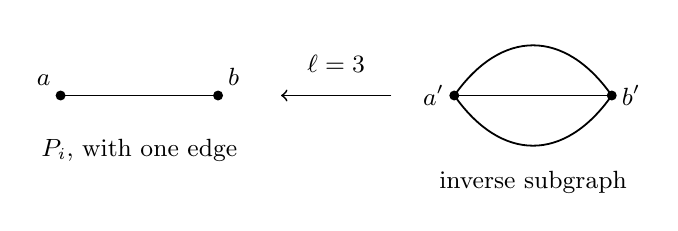
\begin{tikzpicture}[line width=0.65pt, every node/.style={font=\small}]
  \draw (0,0) -- (2,0);
  \fill (0,0) circle (1.8pt) node[above left] {$a$};
  \fill (2,0) circle (1.8pt) node[above right] {$b$};
  \node at (1,-0.7) {$P_i$, with one edge};

  \draw[->] (4.2,0) -- (2.8,0);
  \node at (3.5,0.4) {$\ell=3$};

  \draw (5,0) -- (7,0);
  \draw (5,0) .. controls (5.6,0.85) and (6.4,0.85) .. (7,0);
  \draw (5,0) .. controls (5.6,-0.85) and (6.4,-0.85) .. (7,0);
  \fill (5,0) circle (1.8pt) node[left] {$a'$};
  \fill (7,0) circle (1.8pt) node[right] {$b'$};
  \node at (6,-1.1) {inverse subgraph};
\end{tikzpicture}
